\chapter{Batching Operations for Isogenies}

Our first contribution to the \sidh codebase is the implementation and integration of a procedure for batching together many $\mathbb{F}_{p^2}$ element inversions. This contribution is discussed in detail in the following chapter. The chapter is split into three sections: a high-level discussion of the procedure itself, the low-level details of its integration into \sidh, and finally, the resulting affects of this procedure on the performance of \sidh. 

In the first section of this chapter we will detail the specifics of the partial batched inversion procedure. We will show how the procedure can be constructed by combining two techniques: a well known method for reducing a $\mathbb{F}_{p^2}$ inversion to several $\mathbb{F}_{p}$ operations, and an inversion batching technique outlined in \cite{batching}. 

As we then venture into the lower-level implementation details, we will explore how the procedure can be leveraged optimally in the codebase. We will take a closer look at several of the aforementioned \sidh functions as we illustrate some of the performance bottlenecks in the system. At this time, we will also discuss the design decisions made while implementing the partial batched inversion procedure as well as some of the functions lower-level minutiae.

We will end this chapter by taking a detailed look at the performance gains offered by the inclusion of partial batched inversions in \sidh. More precisely, we will be examining the effects of the procedure on the Yoo et al. signature layer. We will contrast the measured performance of our implementation with an analytical calculation of the expected improvement, and discuss the possible origins of divergent behaviour.  

\section{Partial Batched Inversions}

We will now outline our first contribution to \sidh. The ``partial batched inversion" procedure in question reduces arbitrarily many \emph{unrelated} $\mathbb{F}_{p^{2}}$ inversions to a sequence of $\mathbb{F}_{p}$ operations. The fact that the elements being inverted need not hold any relation will be significant to the applicability of this procedure. For brevities sake, we will henceforth refer to this procedure as \code{pb\_inv}.

As mentioned above, \code{pb\_inv} is constructed by combining two distinct techniques. Both of these techniques improve the efficiency of computing field element inversions: the first is specific to extension fields (in our case, $\mathbb{F}_{p^{2}}$ elements,) but the second is a technique applicable to general field element inversion.

\subsection{$\mathbb{F}_{p^{2}}$ Inversions done in $\mathbb{F}_{p}$}

\subsection{Batching Field Element Inversions}

More specifically, the procedure takes us from \textit{n} $\mathbb{F}_{p^{2}}$  inversions to: 
\begin{center}
\begin{itemize}
\item 2\textit{n} $\mathbb{F}_{p}$ squarings
\item \textit{n} $\mathbb{F}_{p}$ additions
\item 1 $\mathbb{F}_{p}$ inversion
\item 3(\textit{n}-1) $\mathbb{F}_{p}$ multiplications
\item 2\textit{n} $\mathbb{F}_{p}$ multiplications
\end{itemize}
\end{center}

The procedure is as follows:\\

\begin{algorithm}
\caption{Batched Partial-Inversion}\label{euclid}
\begin{algorithmic}[1]
\Procedure{partial\_batched\_inv($\mathbb{F}_{p^{2}}$[ ] vec, $\mathbb{F}_{p^{2}}$[ ] dest, int n)}{}
\State initialize $\mathbb{F}_{p}$ $den[n]$
\For{\texttt{i = 0..(n-1)}}
	\State $den[i] \gets a[i][0]^{2} + a[i][1]^{2}$
\EndFor

\State $a[0] \gets den[0]$

\For{\texttt{i = 1..(n-1)}}
	\State $a[i] \gets \texttt{a[i-1]*den[i]}$
\EndFor

\State $a_{inv} \gets \texttt{inv(a[n-1])}$

\For{\texttt{i = n-1..1}}
	\State $a[i] \gets a_{inv}*dest[i-1]$
	\State $a_{inv} \gets a_{inv}*den[i]$
\EndFor

\State $dest[0] \gets a_{inv}$

\For{\texttt{i = 0..(n-1)}}
	\State $dest[i][0] \gets a[i]*vec[i][0]$
	\State $vec[i][1] \gets -1*vec[i][1]$
	\State $dest[i][1] \gets a[i]*vec[i][1]$
\EndFor
\EndProcedure
\end{algorithmic}
\end{algorithm}


\subsection{Applicability to \sidh}

Because the work of Yoo et al. was built on top of the original Microsoft SIDH library, all underlying field arithmetic (and as such, pointwise arithmetic) is performed in projective space using Montgomery representation. As was mentioned in the previous chapter, doing such allows us to avoid a great deal of field element inversions. We simply convert to Montgomery representation at the beginning of heavy arithmetic, perform the desired operations, and then convert back to standard representation when complete. Throughout the codebase, (most noticeably in \code{kex.c}) we can see an analogous approach taken in for pointwise arithmetic, by first converting to a projective space representation, performing operations, and then converting back to affine coordinates. 

 The downside of this (for our work) is that the number opportunities for implementing the batched inversion algorithm becomes greatly limited.\\

\section{Implementation Details}

\subsection{Parallelizing Signatures}

Because every $2\lambda$ iteration of the \textbf{Sign} and \textbf{Verify} procedures are entirely independent of each other, these functions present themselves as embarrassingly parallel.\footnote{in the field of high performance computing, a problem that is trivially parallizable is often referred to as \emph{embarrassingly} parallizable.} 

Recall from section \ref{subsec:sigcode} the table of functions that can be found in \code{SIDH\_signature}. \code{isogey\_sign} acts as the entry point for \code{Sign} and spawns a POSIX thread for every instance of the for-loop; each one calling \code{sign\_thread} which performs \bob's interaction with \randall. Verification proceeds analogously; \code{isogeny\_verify} is executed and spawns a POSIX threads executing \code{verify\_thread} until all $2\lambda$ iterations are complete.

This parallelization of the signature scheme was the approach taken by Yoo et al. in their original implementation. It also lends itself rather nicely 

\subsection{Security Concerns}

\begin{figure}[htb]
\centering
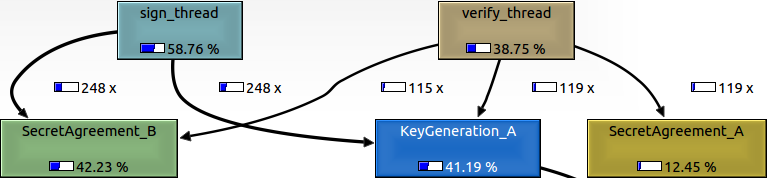
\includegraphics[scale=0.5]{signandverifycall} % e.g. insert ./image for image.png in the working directory, adjust scale as necessary
\caption{<Caption here>}
\label{fig:label} % insert suitable label, this is used to refer to a fig from within the text as shown above
\end{figure}

\section{Results}

Two different machines were used for benchmarking. System A denotes a single-core, 1.70 GHz Intel Celeron CPU. System B denotes a quad-core, 3.1 GHz AMD A8-7600.\\

The two figures below provide benchmarks for KeyGen, Sign, and Verify procedures with both batched partial inversion implemented (in the previously mentioned locations) and not implemented. All benchmarks are averages computed from 100 randomized sample runs. All results are measured in clock cycles.

\begin{center}
\begin{tabular}{@{}lllll@{}}
	\toprule
	Procedure & System A Without Batching & System A With Batching\\
	\midrule
	KeyGen & 68,881,331 & 68,881,331\\
	Signature Sign & 15,744,477,032 & 15,565,738,003\\
	Signature Verify & 11,183,112,648 & 10,800,158,871\\
	\bottomrule
\end{tabular}
\end{center}

\begin{center}
\begin{tabular}{@{}lllll@{}}
	\toprule
	Procedure & System B Without Batching & System B With Batching\\
	\midrule
	KeyGen & 84,499,270 & 84,499,270\\
	Signature Sign & 10,227,466,210 & 10,134,441,024\\
	Signature Verify & 7,268,804,442 & 7,106,663,106\\
	\bottomrule
\end{tabular}
\end{center}

\textbf{System A:} With inversion batching turned on we notice a ~1.1 \% performance increase for key signing and a ~3.5 \% performance increase for key verification.\\

\textbf{System B:} With inversion batching turned on we a observe a ~0.9 \% performance increase for key signing and a ~2.3 \% performance increase for key verification.\\

\subsection{Analysis}

It should first be noted that, because our benchmarks are measured in terms of clock cycles, the difference between our two system clock speeds should be essentially ineffective. \\

In the following table, "Batched Inversion" signifies running the batched partial-inversion procedure on 248 $\mathbb{F}_{p^{2}}$ elements. The procedure uses the binary GCD $\mathbb{F}_{p}$ inversion function which, unlike regular $\mathbb{F}_{p^{2}}$ montgomery inversion, is not constant time.\\

\begin{center}
\begin{tabular}{@{}ll@{}}
	\toprule
	Procedure & Performance \\
	\midrule
	Batched Inversion & 1721718\\
	$\mathbb{F}_{p^{2}}$ Montgomery Inversion & 874178\\
	\bottomrule
\end{tabular}
\end{center}

Do performance increases observed make sense?\\

\subsection{Remaining Opportunities}
There are two functions called in the isogeny signature system that perform a $\mathbb{F}_{p^{2}}$ inversion: j\_inv and inv\_4\_way. These functions are called once in SecretAgreement and KeyGeneration operations respectively. SecretAgreement and KeyGeneration are in turn called from each signing and verification thread.\\

This means that in the signing procedure there are 2 opportunities for implementing batched partial-inversion with a batch size of 248 elements. In the verify procedure, however, there are 3 opportunities for implementing batched inversion with a batch size of roughly ~124 elements.\\

